\documentclass[12pt,a4paper]{article}
\usepackage[utf8]{inputenc} % sempre salve seus arquivos como UTF8
\usepackage[T1]{fontenc}
\usepackage[english]{babel}

\usepackage[left=2.5cm,right=2cm,top=2cm,bottom=2.5cm]{geometry}
\usepackage{amsmath}
\usepackage{amsthm}
\usepackage{amsfonts}

\usepackage{graphicx}
\usepackage{algorithm}
\usepackage{color}
\usepackage[noend]{algpseudocode}
\usepackage{mathtools}
\usepackage{subfig}
\usepackage{diagbox}

% load times font
\usepackage{mathptmx}
\usepackage[scaled=.90]{helvet}
\usepackage{courier}

% comandos
\newcommand{\mdc}[1]{\mathrm{mdc}(#1)}

\DeclarePairedDelimiter\ceil{\lceil}{\rceil}
\DeclarePairedDelimiter\floor{\lfloor}{\rfloor}

% Foot without marker
\newcommand\blfootnote[1]{%
	\begingroup
	\renewcommand\thefootnote{}\footnote{#1}%
	\addtocounter{footnote}{-1}%
	\endgroup
}

\title{MO446 -- Introduction to Computer Vision  \\ Project 2}
\author{Breno Leite  \\ Guilherme Leite}
\date{29/08/2017}

\begin{document}

\maketitle
\blfootnote{\textit{\textbf{Important note:} The borders seen in the figures are not part of the image, they are figurative information about the starting and ending points of the image. Moreover, all the image scales in this report were changed in order to make the text more readable.}} \\

%% ---------------- Starts here --------------------------------

\textbf{\LARGE Input Images}\\


\begin{figure}[!h]
	\centering
	\subfloat[Face to be blended (\textbf{p1-2-4-3})]{
		{
			\setlength{\fboxsep}{1pt}
			\setlength{\fboxrule}{1pt}
			\fbox{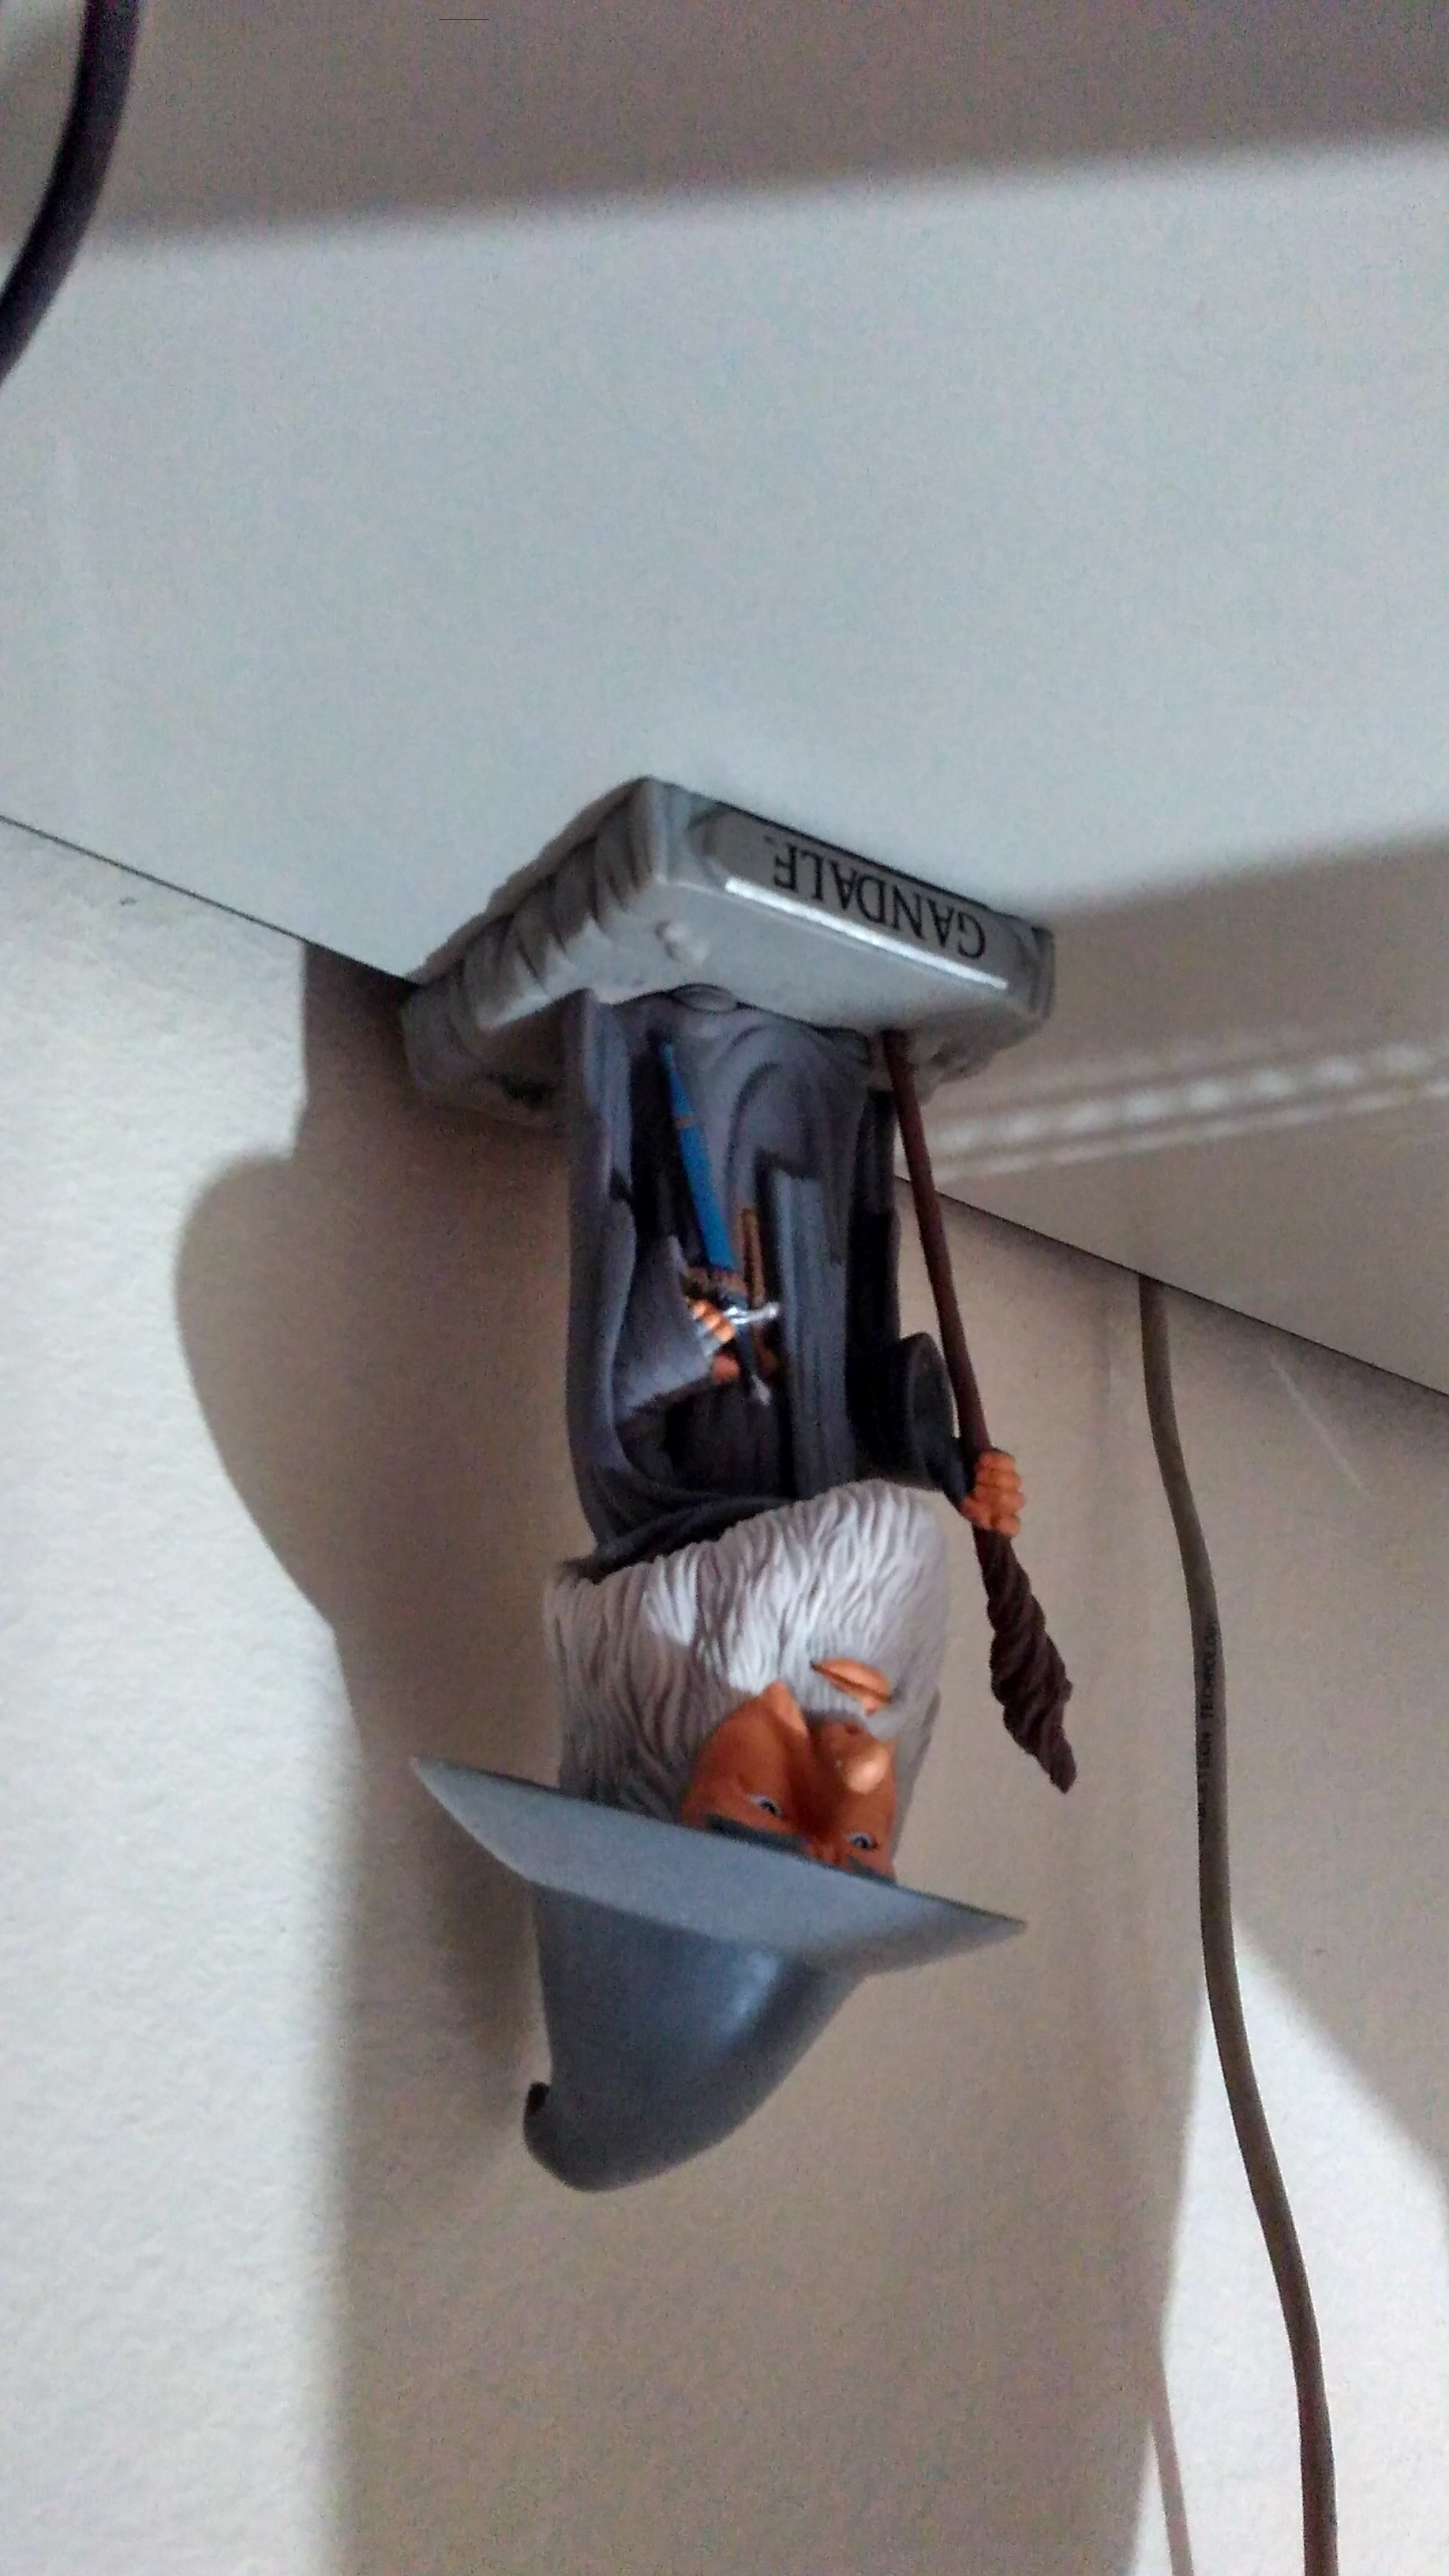
\includegraphics[scale=0.35]{input/img1}}
		}
	}
	\quad
	\subfloat[Hand to be blended (\textbf{p1-2-4-4})]{
		{
			\setlength{\fboxsep}{1pt}
			\setlength{\fboxrule}{1pt}
			\fbox{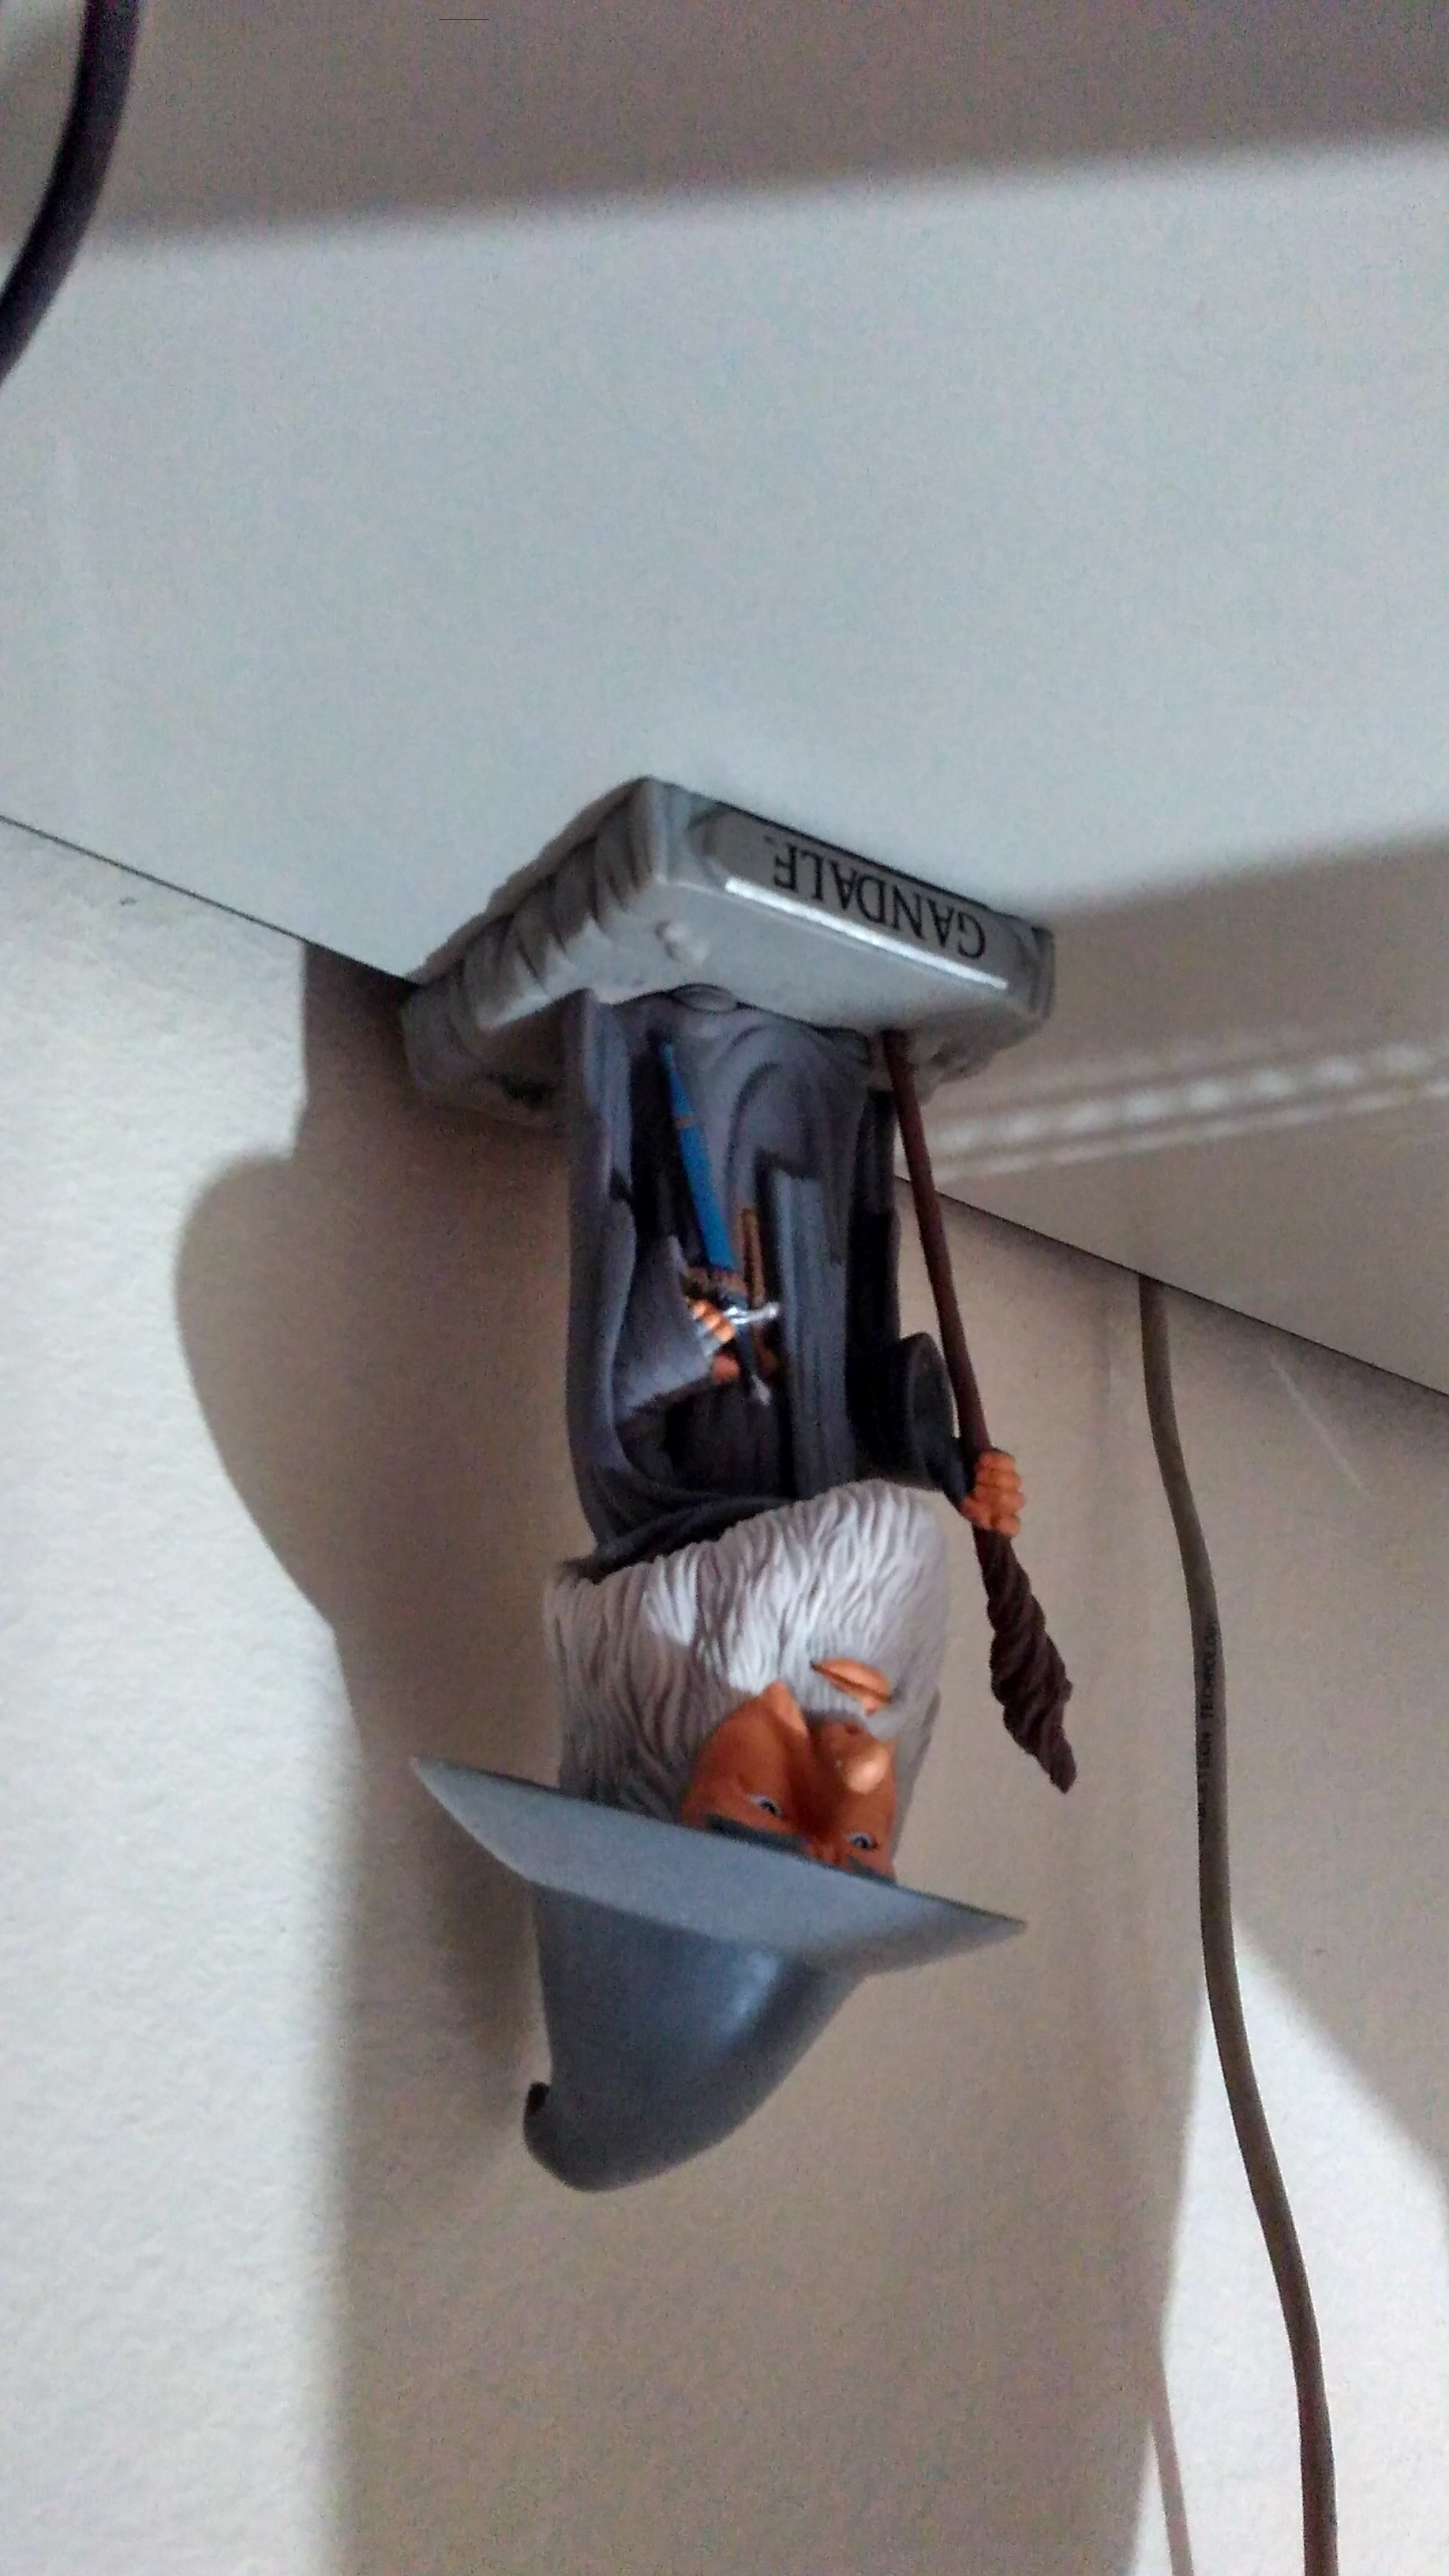
\includegraphics[scale=0.35]{input/img1}}
		}
	}
	\caption{Complementary images used for further testing the blending operations.}
	\label{fig:blendingFurther}
\end{figure}

\begin{figure}[!h]
	\centering
	{%
		\setlength{\fboxsep}{1pt}%
		\setlength{\fboxrule}{1pt}%
		\fbox{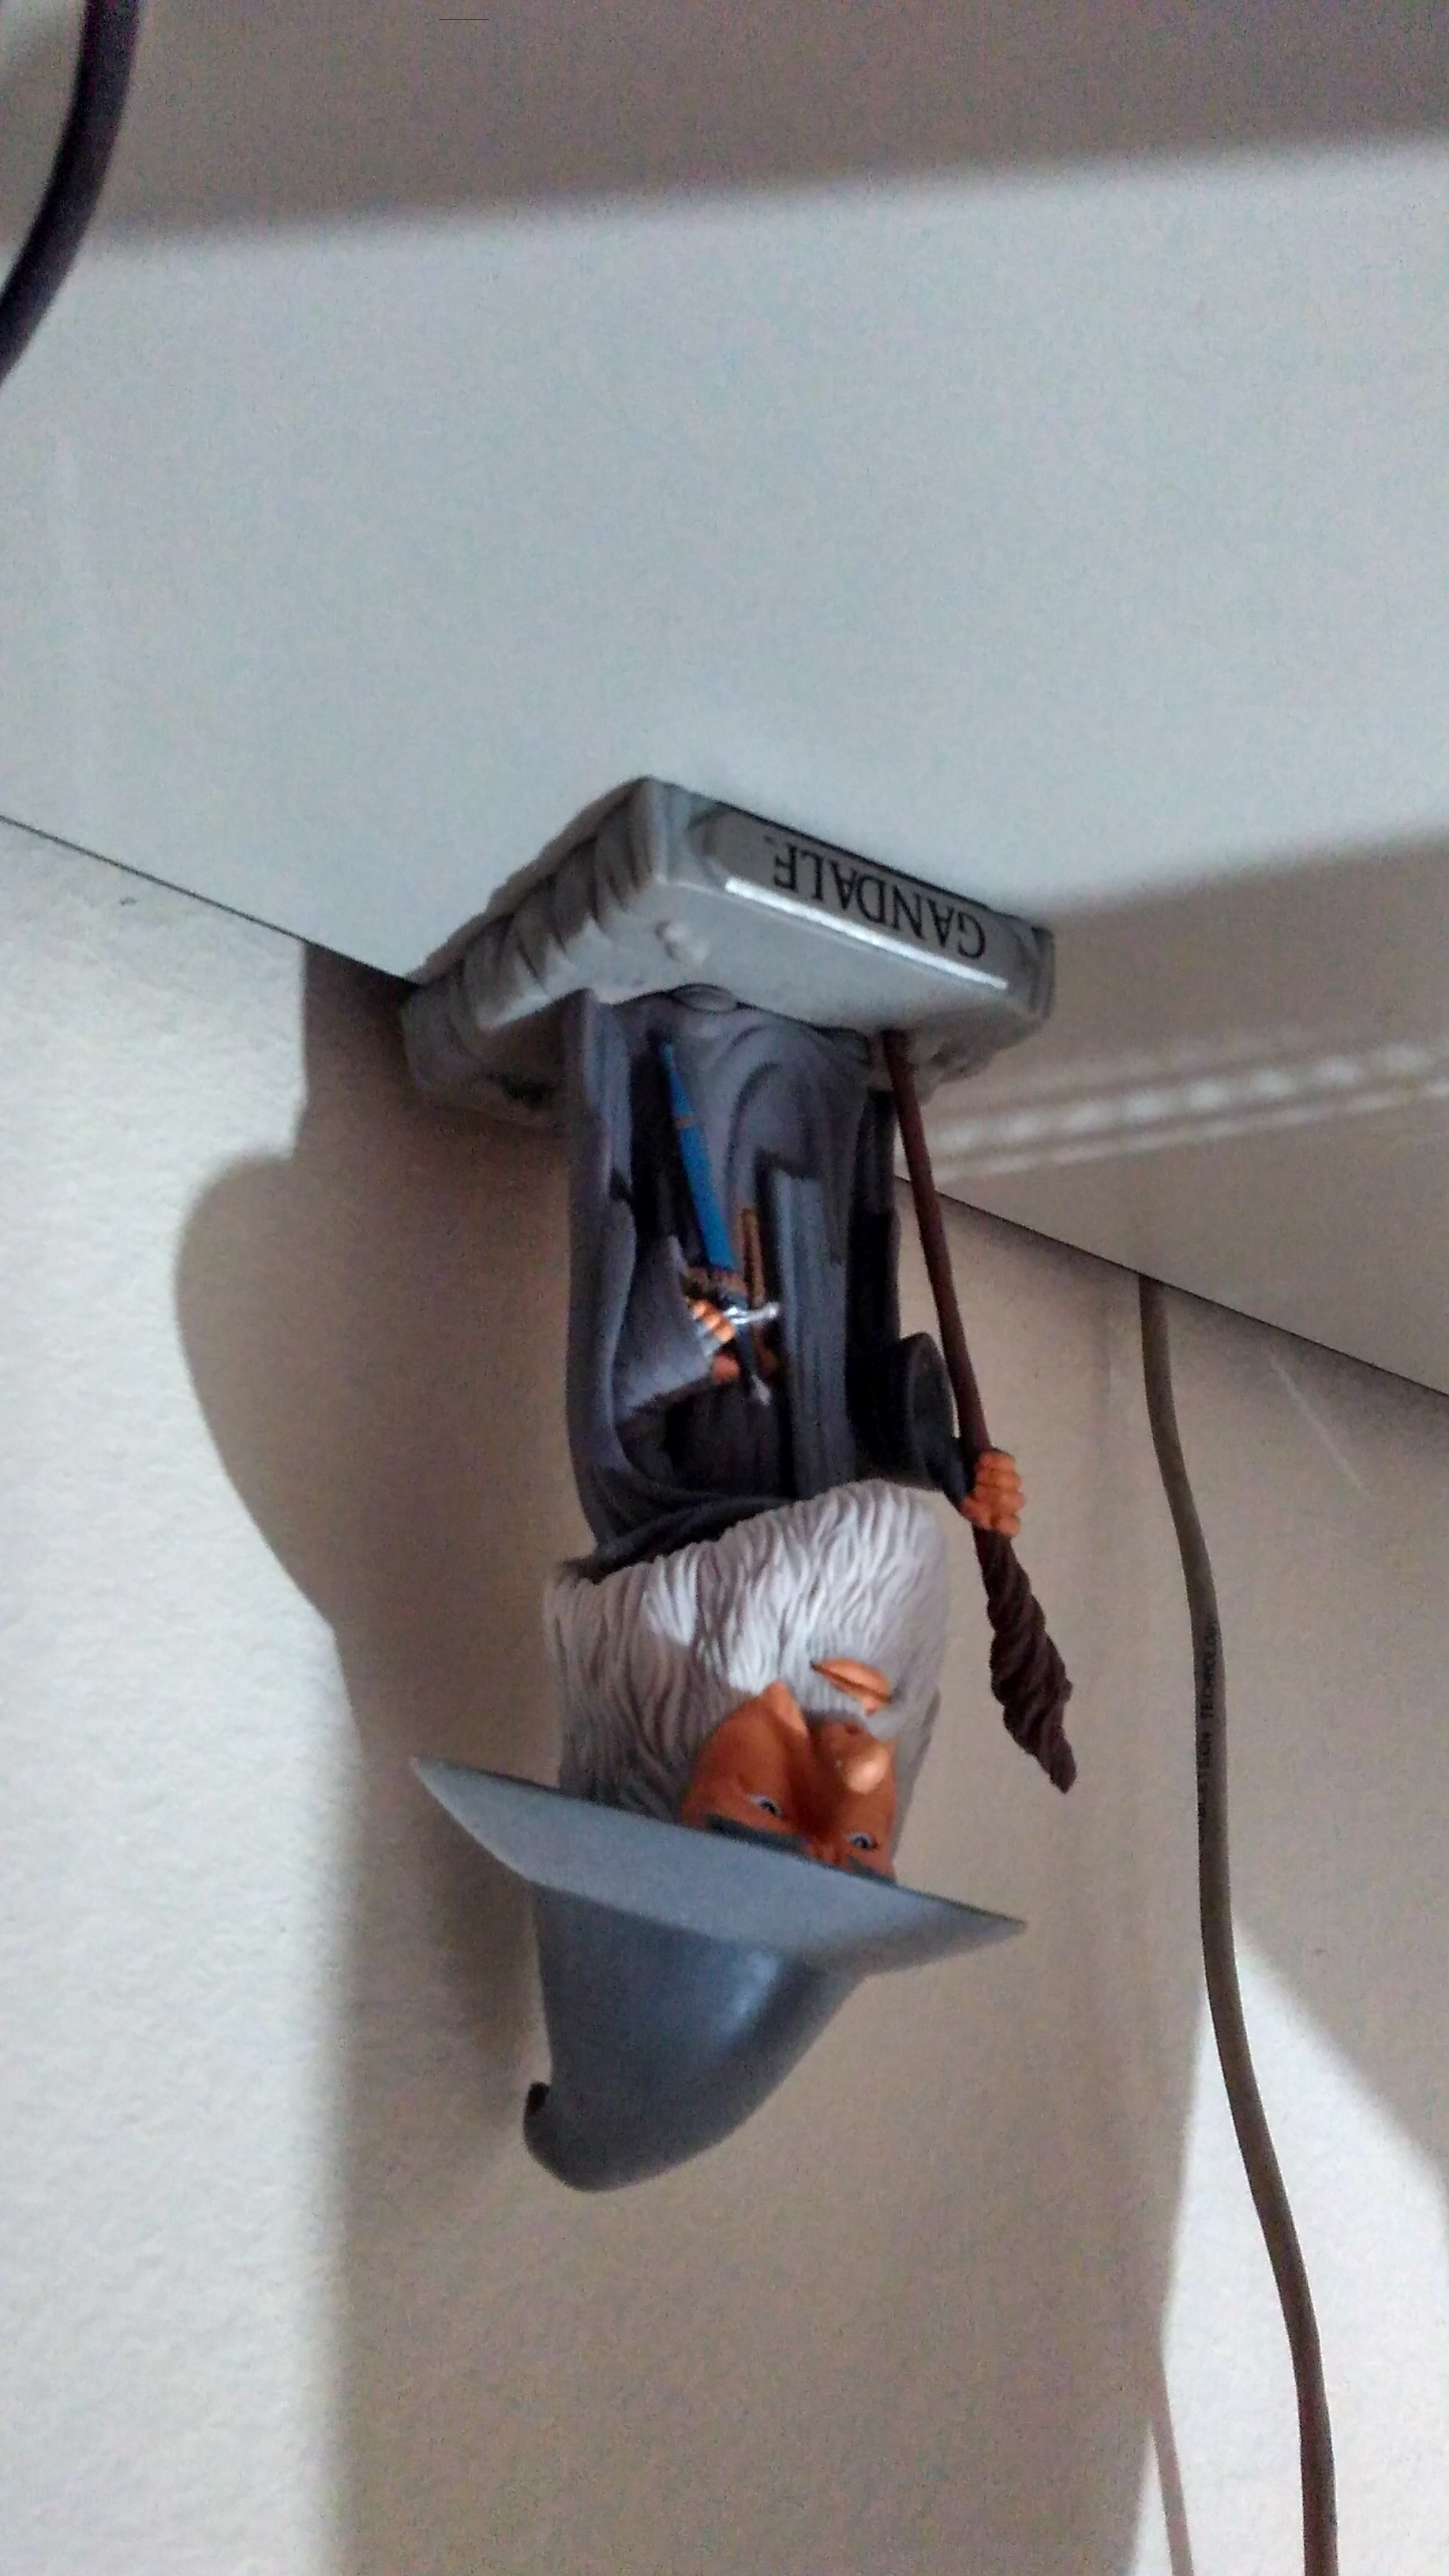
\includegraphics[scale=0.55]{input/img1}}%
	}%
	\caption{Reconstructed image from inverse Fourier transform using 100\% of pixels in magnitude and phase. (\textbf{p1-3-1-6, p1-3-1-11, p1-3-1-16, and p1-3-1-21})}
	\label{fig:inverse}
\end{figure}


\end{document}
